% Here you can see how to include an image in your document.

% \begin{sidewaysfigure}
% \centering
% 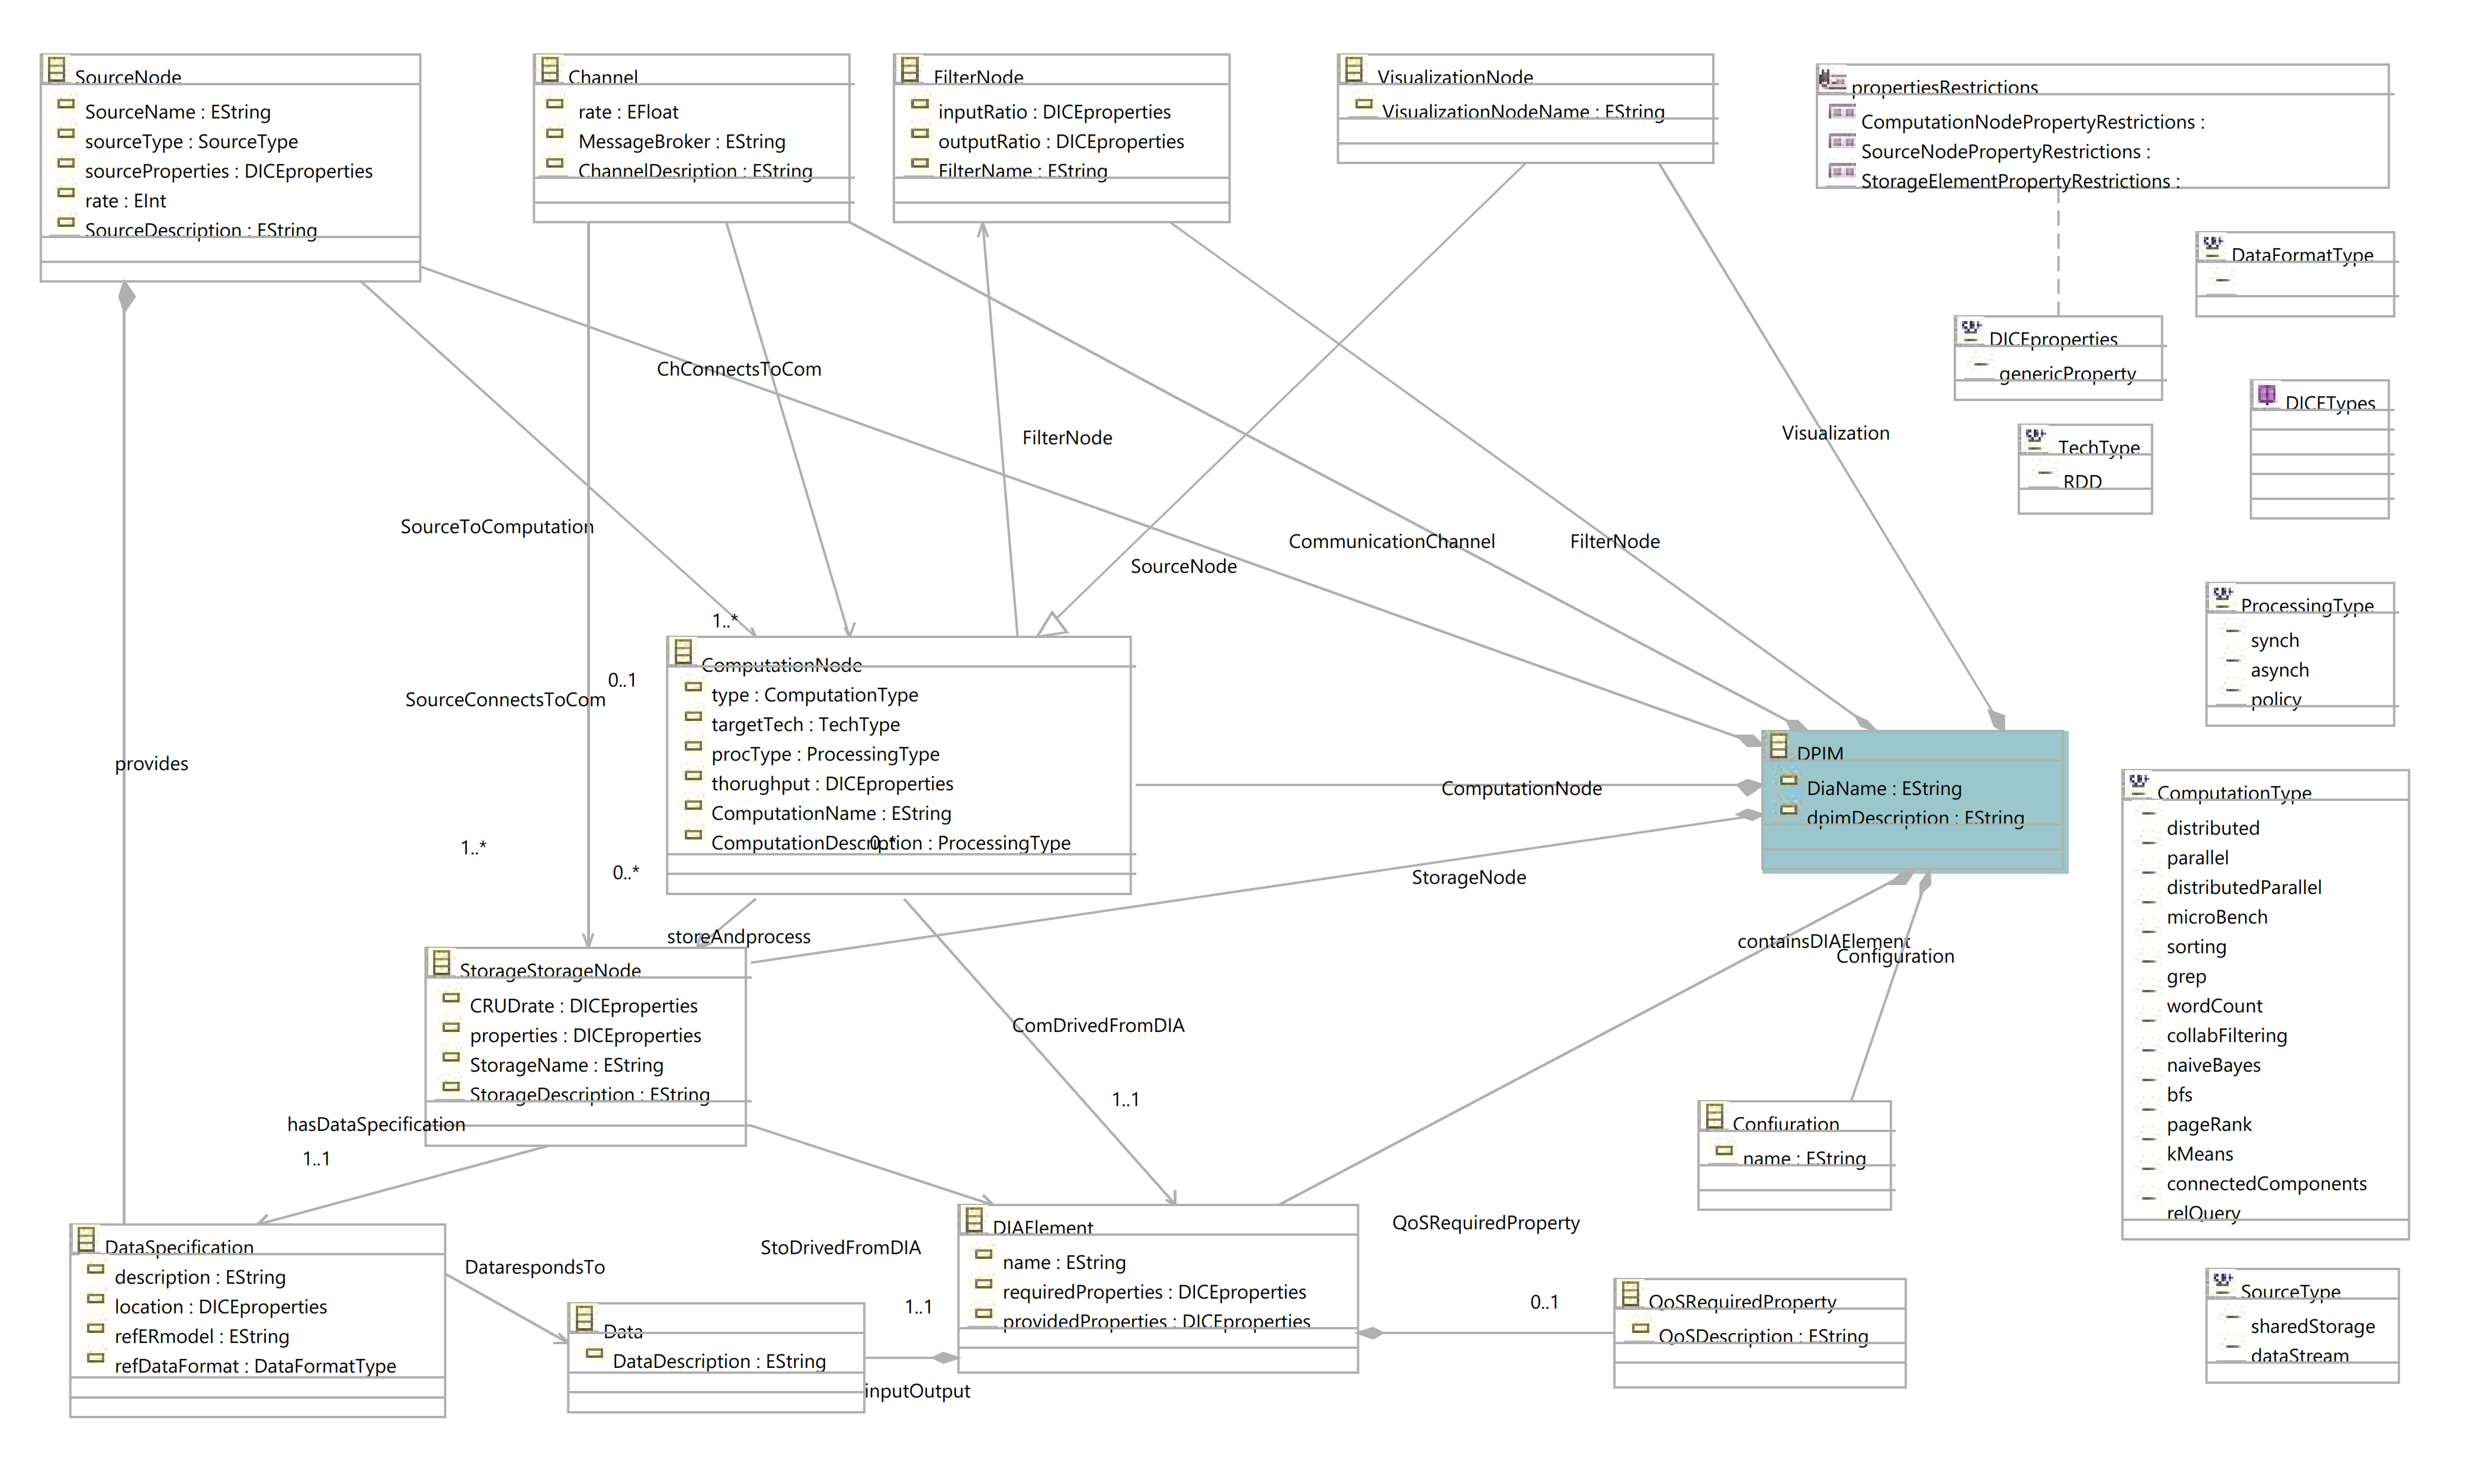
\includegraphics[width=\textwidth]{Images/11.png}
% \caption{\label{fig:metamodel}DICE DPIM metamodel.}
% \end{sidewaysfigure}

% \begin{figure}
% \centering
% 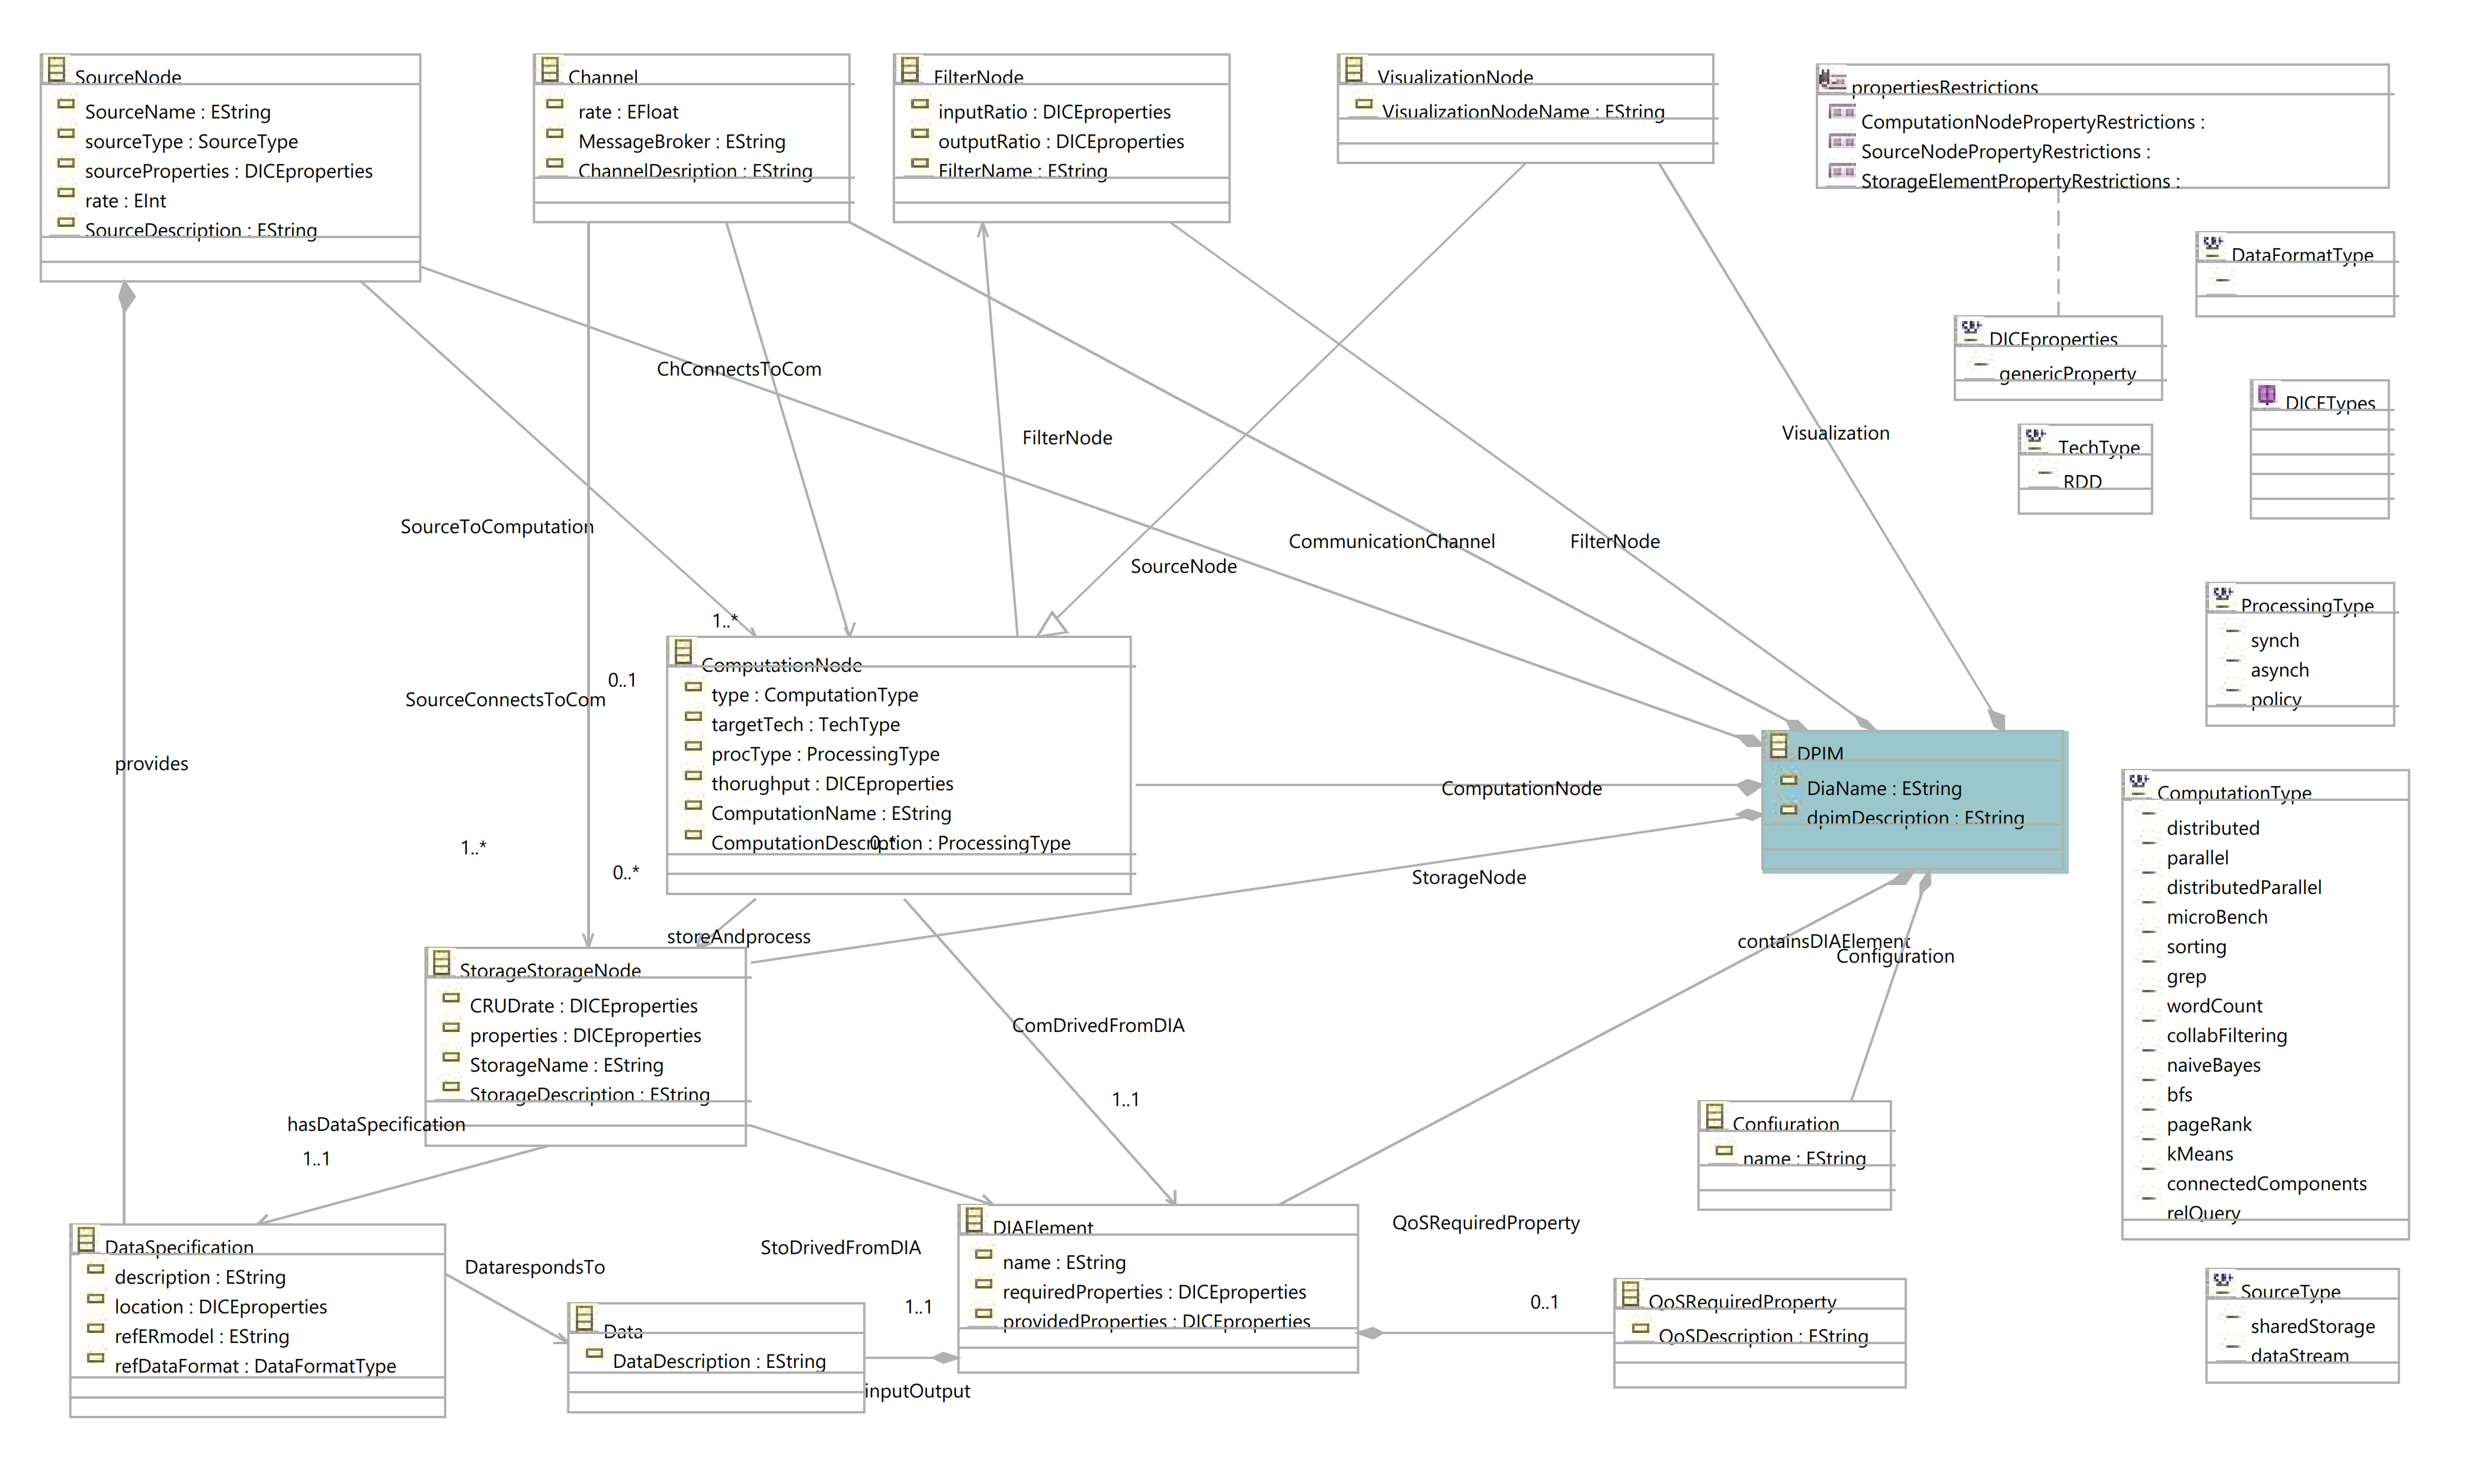
\includegraphics[width=\textwidth]{Images/11.png}
% \caption{\label{fig:metamodel2}DICE DPIM metamodel in portrait form.}
% \end{figure}

% Here is the command to refer to another element (section, figure, table, ...) in the document: \emph{As discussed in Section~\ref{sect:overview} and as shown in Figure~\ref{fig:metamodel}, ...}. Here is how to introduce a bibliographic citation~\cite{DAM}. Bibliographic references should be included in a \texttt{.bib} file. 

% Table generation is a bit complicated in Latex. You will soon become proficient, but to start you can rely on tools or external services. See for instance this \href{https://www.tablesgenerator.com}{https://www.tablesgenerator.com}. 
\subsection{Product Perspective}
\subsubsection{Scenarios}

\textbf{Student registers in the platform}

Dwight Schrute decides it's about time to get an internship, so he opens his notebook and acesses the S\&C website. Once acessed, the site offers a login page in which he clicks the ``New account'' button and is redirected to a page in which he fills his personal and contact information and uploads his CV. Once he is done with the form, S\&C checks the filling of all mandatory data, as well as the correctness of information (existing email, legal age, etc). A confirmation email is sent to his adress and, once confirmed, his account is registered and he can use it to login. Also, a profile is set to him according to his personal information and CV, which can be used later to recommendations.


\textbf{Publish new internship}

Toby, an HR representative at Dunder Mifflin Paper Company, is informed that the digitizations of assets project needs an intern. He meets up with the manager of the project to determine the requirements and responsibilities of the role. They also define the questionnaire interviewers will need to use to asses candidates during interviews. Then, he meets with the head of HR to refine the compensation package they will offer. With all the information, Toby navigates to S\&C in his browser. He logs in, clicks on ``New Internship Position'' and fills all the required details (skills, experience, compensation, benefits, duration and tasks-to-be-performed). Then he clicks the ``Save and Publish'' button. 

S\&C validates the inputted information. If it is not valid, it prompts Toby to correct it. Otherwise, it saves the position details and publishes the announcement. Toby sees a pop-up in his screen confirming that the position has been created successfully. 

 
\textbf{Cancel an open internship}

Francis is made aware by his boss that the internship position he’s looking to recruit for needs to be closed due to budget cuts in the company. He navigates to S\&C, logs in and clicks on ``Open internships''. There, he selects the aforementioned internship and clicks on ``Cancel Internship''. A pop-up appears on the screen asking for confirmation. He clicks on “Confirm”. 

 
\textbf{Student proactively looks for an internship}

Dwight opens the S\&C website to look for an internship. The website pops a login page, in which he enters his credentials and acesses the platform. Once logged in, he searches the internship of his dreams to better suit his needs, specifying filters such as work position, geographical location, available programs, companies of preference etc. He finds Dunder Mifflin Paper Company and clicks on one of their internship programs, expanding his view to all of the project’s provided information (duration, technologies used, benefits, payment…) in its main page. Given his enthusiasm on the internship offer, he clicks the easy-application button and S\&C register his application by adding him to the applicants poll. 

 
\textbf{S\&C matchmakes internships and students}

After the publication of Dunder Mifflin Paper Company internship position, S\&C runs its matching algorithm and finds a high suitability for Jim Halpert’s profile. He receives a notification email communicating him from the new opened position that might interest him and his account is added to the list of potential suitable profiles, available to Dunder Mifflin Paper Company.

 
 
\textbf{Schedule an interview}

Holly, the Hiring Manager of the Bomb Project at ACME, is notified through an email from S\&C that a new candidate applied for the internship she published two days ago. She then clicks on the link provided in the email and is redirected to the web-app S\&C, where she logs in and then reviews said candidate’s CV. She thinks the student might be a great fit for the role, so she clicks on the “Schedule an interview” button that appear right next to the candidate’s description.

A pop-up comes up prompting her to input her availability for the week and the desired interview duration for this candidate. She provides her schedule and clicks on “Save”.

 
\textbf{S\&C invites the candidate, Ryan, to an interview}

Ryan receives an email from S\&C inviting him to an interview for an internship he applied to. He clicks on the “Find a time” button. 

He is redirected to the S\&C website, where he logs in and is met with possible times for said interview. S\&C only shows the available times Holly provided. Ryan chooses Tuesday afternoon, as he does not have classes that day. He then clicks on “Confirm Assistance”.

S\&C schedules the interview and notifies the interviewer. Ryan is informed that his interview has been scheduled correctly.

\textbf{Carry on an interview}

Anna has an interview scheduled with Michael. He arrives on time to the office, Anna greets him and takes him to the conference room for the interview. She opens S\&C, logs in, and looks for the “Coffee Server Internship”, a customized questionnaire that her company uploaded to S\&C to conduct interviews for this role. She conducts her interview in her own style, rephrasing the questions from the questionnaire but extracting the key information. She takes notes of Michael’s answers and fills the questionnaire.

When Anna has all the information she needs to fill the questionnaire, she asks Michael if he has any questions. After he says no, she says goodbye and leads him to the exit. The interview finishes. Anna then goes back to her notes and reviews the questionnaire before saving it. When she clicks on “Save”, she is prompted to input a verdict (approve or reject) for Michael. The interview was good and Michael seemed really for for the role. She clicks on “Approve”. To submit the approval, S\&C asks her to provide the start date, time and place of the internship for Michael.

S\&C saves the interview as successful and notifies Michael about the good news. It also provides information about the start date, time and place of the internship.

 
    \textbf{Complain about an internship}

Gianna, the leader of the “Butterfly Effect” research project, is worried because the team is not getting along with the new intern. So she navigates to S\&C platform in her browser, logs in,  and clicks on the “Ongoing internships” tab. There, she selects the one that is causing trouble and then clicks on “Create Complaint”. A form pops-up asking her to provide a detailed description of the issue. She describes the issue and clicks on “Send”.

S\&C receives the complain and triggers a process involving the university to handle it (out of the project’s scope).

\textbf{The company provides a feedback to a finished internship}

John receives an email from S\&C asking for his feedback on past semester’s intern, Lorena. He is really happy with the work she’s done, and believes she might be a great fit for a full time position in the future. He clicks on the “Give feedback” button and is redirected to the S\&C app, where he logs in and is faced with four questions arranged on a form:

\begin{enumerate}
    \item How would you rate Lorena’s performance from one to ten?
    \item (Optional) Any comments on this internship in particular?
    \item (Optional) How would you rate your experience with S\&C from one to ten?
    \item (Optional) Any comments, feedback or suggestions on the platform?
\end{enumerate}

He fills the questionnaire and clicks on “Submit”

S\&C saves the data for statistical analysis.
 

\textbf{The student provides feedback to a finished internship}

Lorena receives an email from S\&C asking for her feedback on her recent internship at Dunder Mifflin. She is really happy with the experience and feels she learned a lot, especially in terms of project management and teamwork. She clicks on the “Give feedback” button and is redirected to the S\&C app, where she logs in and is faced with four questions arranged on a form:

\begin{enumerate}
    \item How would you rate your overall experience from one to ten?
    \item (Optional) Any comments on this internship in particular?
    \item (Optional) How would you rate your experience with S\&C from one to ten?
    \item (Optional) Any comments, feedback or suggestions on the platform?
\end{enumerate}

She fills out the questionnaire and clicks on “Submit.”

S\&C saves the data for statistical analysis.
\textbf{User looks at their analytics data}

Julian is preparing a mid-Q report on the hiring team’s performance. He opens the S\&C web-app, logs in and enters the “Analytics” tab. There, he is able to see three main metrics:

\begin{enumerate}
    \item Interest \%: Amount of students that applied over amount of students that saw an internship details for Julian’s company.
    \item Approval \%: Students that approved the interview over students that had interviews scheduled
    \item  Company NPS: Median feedback rate given to the company by students that completed internships position within it.
\end{enumerate}

He analyzes the metrics over time and takes a screenshot for a company presentation on the hiring processes.
\clearpage
\subsubsection{Domain Class Diagram}

Here we include the Domain Level Class Diagram, focusing on key entities such as students, companies, internships, and feedback. These elements represent the core interactions within the platform and align closely with the project's goals of facilitating student-internship matches and supporting the selection process.

We prioritized simplicity and relevance by modeling only essential relationships, such as applications, recommendations, and interview processes. This ensures the diagram remains clear and actionable for both development and analysis, avoiding unnecessary complexity.

The precise modeling of classes like WorkProfile, InterviewQst, Slot, and RecommenderSystem has been deferred to the design stage. This decision allows flexibility, as various implementations can satisfy the requirement specifications while adapting to different design needs.

\begin{figure}[htbp]
\centering
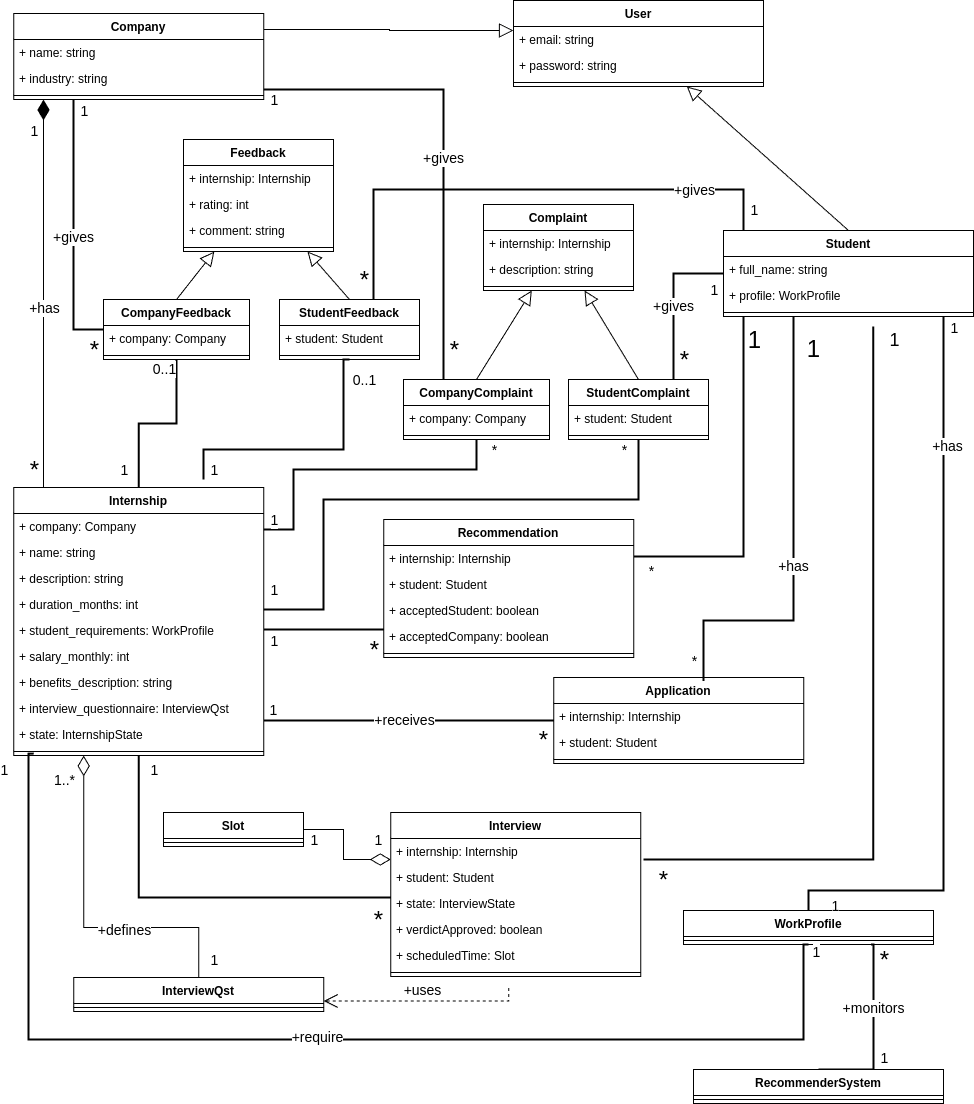
\includegraphics[scale=0.45]{Images/class-diagram.png}
\caption{\label{fig:class-diagram} Domain Level Class Diagram}
\end{figure}

\subsubsection{State Diagrams}

We chose to diagram interviews and internships because they are central entities in the selection process, representing its key stages. The states of these entities encapsulate the primary interactions between students and companies, making them essential to understand the overall workflow.

By focusing on these entities, we aimed to bring clarity to the reader by illustrating the core elements of the process. Their states naturally reflect the possible actions and outcomes, making them ideal candidates for state modeling and providing a structured view of the selection system.

\begin{figure}[H]
\centering
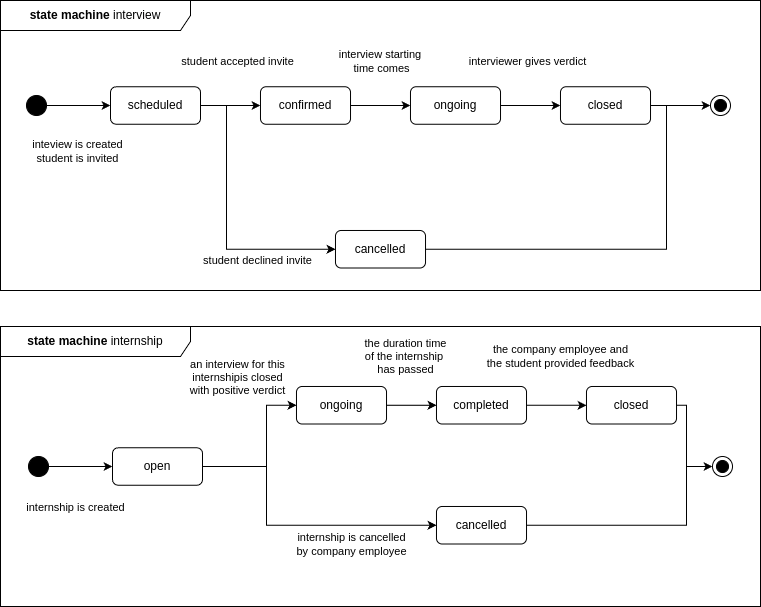
\includegraphics[width=\textwidth]{Images/state_diagrams.png}
\caption{\label{fig:state-diagrams} State Diagrams}
\end{figure}
\subsection{Product Functions}
\textbf{Sign-Up, Login, and Profile Management}

This function allows students and companies to sign up, log in, and manage their profiles on the platform. Upon signing up, students upload their CVs, which are used to create their profiles, while companies provide relevant organizational information. This function verifies the provided data (e.g., email, legal age) to ensure it meets platform requirements. Once registered, users can log in, update their information, and track their internship applications or postings.

\textbf{Internship Publication and Management}

This function allows companies to publish new internship positions, edit existing ones, and cancel open internships. Companies provide details such as required skills, tasks, compensation, and benefits, which are validated for correctness and completeness. Once published, the internship is visible to students. If necessary, companies can also manage ongoing internships by editing or canceling them, keeping the platform’s listings up to date.

\textbf{Search and Apply for Internships}

This function allows students to search for internships based on various criteria such as role, location, and compensation. Students can apply to internships with a single click, adding themselves to the list of applicants. The platform also sends proactive notifications to students about relevant opportunities, based on their profile data and past behaviors.

\textbf{Internship Matching and Recommendation}

This function allows the platform to recommend internships to students and suggest student profiles to companies based on matching criteria. The matching algorithm evaluates student profiles and internship details to suggest suitable opportunities. It continuously refines recommendations using data from student interactions (such as applications) and feedback from companies. The system sends notifications to both parties about suitable internships or candidates.

\textbf{Interview Management and Selection Process}

This function allows companies to schedule interviews with students, manage interview details, and track candidate progress. Companies provide available time slots, and students confirm their attendance. During interviews, companies use custom questionnaires to assess candidates, recording feedback in the platform. Afterward, companies decide whether to approve or reject candidates, and the platform tracks the outcome, notifying both parties about the decision.

\textbf{Feedback and Complaint Management}

This function allows students and companies to provide feedback on internship experiences and raise complaints during ongoing internships. After internships conclude, companies rate students' performance, while students rate their overall experience. The platform uses this feedback to improve future internship matches. If issues arise during an internship, either students or companies can file complaints, which are then handled by the platform, often involving university representatives for resolution.

\textbf{Internship Analytics and Reporting}

This function allows companies and the platform to track and analyze various metrics related to internships. Metrics such as application rates, interview success rates, and feedback scores are collected to evaluate and improve the internship process. This data also feeds into the recommendation system, enhancing the quality of future matches between students and internships. Companies can view performance reports and adjust their recruitment strategies accordingly.
\subsection{User characteristics}

\textbf{Student}

The student is a user who creates and manages their profile, including uploading their CV, providing personal and academic details, and specifying internship preferences. Students can search for available internships, apply to positions, and receive notifications about opportunities that match their profiles. They can view internship details, track their applications, and receive interview invitations. After completing an internship, students can provide feedback on their experience and file complaints about ongoing internships if needed. Based on their profiles and activities, students are matched with relevant internship opportunities through the platform’s recommendation system. The student’s role focuses on searching for, applying to, and managing internship applications, participating in interviews, and engaging in feedback processes.

\textbf{Company}

The company user can create and manage their organizational profile, as well as publish internship listings. They provide details such as required skills, tasks, compensation, benefits, and other terms. Companies can edit, cancel, or close internship listings as necessary. They are responsible for reviewing student applications, selecting candidates, scheduling interviews, and conducting interviews using custom questionnaires. Once an internship is completed, companies can provide feedback on the student’s performance. Companies also have the option to file complaints about ongoing internships if issues arise. Additionally, they can access analytics to monitor the recruitment process, track key metrics like application success rates, interview outcomes, and student feedback, and evaluate the overall performance of their internship programs.
\subsection{Assumptions, Dependencies and Constraints}
\subsubsection{Domain Assumptions}
    \begin{enumerate}[label={[DA\arabic*]}]
        \item Users provide accurate and up-to-date information to the platform.
        \item Students have a CV and a notion of their skills and profile.
        \item Companies have a detailed notion of the internship position and the profile they are hiring for.
        \item Internships are temporal contracts with explicit deadlines .
        \item Companies have a pre-defined process for hiring that involves interaction with S\&C.
        \item The company user sticks to the company-defined hiring process through the platform.
        \item Users interested in setting-up interviews know in advance their availability for the week.
        \item Every user has a valid email account that they check at least once every 48 hours.
        \item Email communication is regarded by users as a reliable channel for work-related information.
        \item Students are proactively interested in getting an internship.
        \item Users remember their authentication credentials
    \end{enumerate}
